\documentclass[conference]{IEEEtran}
\IEEEoverridecommandlockouts
% The preceding line is only needed to identify funding in the first footnote. If that is unneeded, please comment it out.
\usepackage{booktabs}
\usepackage{lastpage}
\usepackage{float}
\usepackage{cite}
\usepackage{lastpage}
\usepackage[hidelinks]{hyperref}
\usepackage{amsmath,amssymb,amsfonts}
\usepackage{algorithmic}
\usepackage{graphicx}
\usepackage{textcomp}
\usepackage{xcolor}
\def\BibTeX{{\rm B\kern-.05em{\sc i\kern-.025em b}\kern-.08em
    T\kern-.1667em\lower.7ex\hbox{E}\kern-.125emX}}
\begin{document}

\title{A Stacked Ensemble Learning Approach for Hyper-Local PM2.5 Prediction Using Satellite AOD and Meteorological Data\\}

\author{\IEEEauthorblockN{1\textsuperscript{st} Md. Masum Billah}
\IEEEauthorblockA{\textit{Department of Computer Science and Engineering} \\
\textit{Bangladesh University of Business and Technology (BUBT)}\\
Dhaka, Bangladesh \\
md.masum.cse.bd@gmail.com}
\and
\IEEEauthorblockN{2\textsuperscript{nd} Md. Syfulla}
\IEEEauthorblockA{\textit{Department of Computer Science and Engineering} \\
\textit{Bangladesh University of Business and Technology (BUBT)}\\
Dhaka, Bangladesh \\
syfullasanto122@gmail.com}
\and
\IEEEauthorblockN{3\textsuperscript{rd} Chowdhury Kashfee Kamal Fagun}
\IEEEauthorblockA{\textit{Department of Computer Science and Engineering} \\
\textit{Bangladesh University of Business and Technology (BUBT)}\\
Dhaka, Bangladesh \\
kashfee368@gmail.com}
\and
\IEEEauthorblockN{4\textsuperscript{th}Tanveer Rabbani}
\IEEEauthorblockA{\textit{Department of Computer Science and Engineering} \\
\textit{Bangladesh University of Business and Technology (BUBT)}\\
Dhaka, Bangladesh \\
tanveerrabbani2002@gmail.com}
\and
\IEEEauthorblockN{5\textsuperscript{th} Md. Jahidul Islam}
\IEEEauthorblockA{\textit{Department of Computer Science and Engineering} \\
\textit{Bangladesh University of Business and Technology (BUBT)}\\
Dhaka, Bangladesh \\
jahidislam1204.bd@gmail.com}

}

\maketitle

\begin{abstract}
Accurate hyper-local estimation of fine particulate matter (PM$_{2.5}$) is essential for effective air quality management but is constrained by the sparse spatial coverage of ground-based monitoring stations. This study proposes an ensemble-based machine learning framework that integrates ground-level PM$_{2.5}$ measurements with satellite-derived Aerosol Optical Depth (AOD), meteorological variables, and geospatial information. Random Forest and XGBoost regressors are employed as complementary base learners, and their predictions are combined using a linear regression--based meta-model to produce final PM$_{2.5}$ estimates. Evaluation on a held-out test set shows that the ensemble model achieves an $R^2$ value of approximately $0.56$, outperforming individual base models and demonstrating the effectiveness of ensemble learning in data-scarce environments. Feature importance analysis highlights the dominant influence of satellite-derived AOD and spatial location. Furthermore, the trained model is deployed as a real-time Flask-based application programming interface (API) that integrates live meteorological data to provide instantaneous PM$_{2.5}$ predictions and corresponding Air Quality Index (AQI) categories, illustrating its practical applicability for hyper-local air quality estimation.
\end{abstract}

\begin{IEEEkeywords}
PM$_{2.5}$ prediction, ensemble learning, Aerosol Optical Depth, Air Quality Monitoring, Machine Learning, Heterogeneous data fusion, Random Forest, XGBoost.
\end{IEEEkeywords}


\section{INTRODUCTION}

Air quality degradation has emerged as a major environmental and public health concern worldwide, particularly in rapidly urbanizing and industrializing regions \cite{b1,b2}. Increased emissions from transportation, industrial activities, and energy consumption have significantly elevated atmospheric pollution levels, posing serious risks to human health and environmental sustainability. Consequently, accurate monitoring and prediction of air pollutant concentrations are essential for effective air quality management and evidence-based policy-making.

Among atmospheric pollutants, fine particulate matter (PM$_{2.5}$) is considered one of the most harmful due to its ability to penetrate deep into the respiratory system and enter the bloodstream. Prolonged exposure to PM$_{2.5}$ has been strongly associated with cardiovascular and respiratory diseases, premature mortality, and reduced life expectancy, making reliable estimation and forecasting of PM$_{2.5}$ concentrations a critical research problem.Recent advances in machine learning and deep learning have significantly improved air quality prediction performance. Prior studies and surveys \cite{b1,b2} demonstrate that data-driven models can effectively capture complex nonlinear relationships in air quality data. Deep learning architectures, including recurrent, attention-based, and hybrid spatiotemporal models, have shown strong predictive capabilities for PM$_{2.5}$ forecasting \cite{b3,b4,b5,b6,b7,b8}. However, these approaches often require large volumes of high-quality data, dense monitoring networks, and substantial computational resources, limiting their applicability in data-scarce regions and real-time operational settings.

To address the limitations of ground-based monitoring, satellite remote sensing has been widely adopted as a complementary data source for air quality assessment. Satellite-derived Aerosol Optical Depth (AOD) provides valuable information on atmospheric aerosol loading and has been extensively used to estimate surface-level PM$_{2.5}$ concentrations \cite{b9,b10}. Integrating AOD with meteorological and geographic variables has been shown to improve spatial coverage and estimation accuracy, particularly in regions with sparse monitoring infrastructure.
Tree-based machine learning models, such as Random Forests and XGBoost, have proven effective for satellite-based PM$_{2.5}$ estimation due to their ability to model nonlinear relationships and handle heterogeneous data \cite{b11,b12,b13}. More recently, ensemble learning and stacked generalization techniques have gained attention for further improving prediction robustness and generalization performance \cite{b14,b15}. Despite these advances, existing studies often focus on offline modeling and lack deployment-ready solutions that support hyper-local estimation and real-time inference.

Motivated by these challenges, this study proposes an ensemble-based framework for hyper-local PM$_{2.5}$ estimation that integrates ground-based observations, satellite-derived AOD, meteorological variables, and geographic information. The proposed approach combines Random Forest and XGBoost regressors within a stacked learning architecture to enhance predictive accuracy and robustness while maintaining computational efficiency. Furthermore, the framework is implemented as a real-time Flask-based API, demonstrating its suitability for operational air quality monitoring and decision support.


The main contributions of this work are summarized as follows:
\begin{itemize}
\item We propose a multi-source data fusion framework that integrates ground-based PM$_{2.5}$ measurements, satellite-derived AOD, meteorological variables, and geographic information for hyper-local air quality estimation.
\item We develop a stacked ensemble learning model combining Random Forest and XGBoost regressors with a linear regression meta-learner, achieving improved predictive performance over individual models.
\item We conduct a feature importance analysis to identify the key factors influencing surface-level PM$_{2.5}$ concentrations.
\item We implement the proposed framework as a real-time Flask-based API using live meteorological data, demonstrating its applicability for operational air quality monitoring.
\end{itemize}

The remainder of this paper is organized as follows. 
\hyperref[sec:literature]{Section~II} reviews related work on PM$_{2.5}$ prediction, satellite-based air quality estimation, and ensemble learning approaches. 
\hyperref[sec:methodology]{Section~III} describes the materials and methodology, including data sources, preprocessing steps, model architecture, and training procedures. 
\hyperref[sec:deployment]{Section~IV} presents the system deployment structure and operational workflow of the proposed framework. 
\hyperref[sec:results]{Section~V} results along with performance evaluation and analysis. 
Finally, \hyperref[sec:conclusion]{Section~VI} concludes the paper and outlines directions for future research.






\section{Literature Review}
\label{sec:literature}

Méndez et al. \cite{b1} presented a comprehensive survey of machine learning techniques for air quality forecasting published between 2011 and 2021. The study compared traditional regression models and deep learning approaches, concluding that LSTM-based models better capture temporal dependencies in pollutant data, while highlighting challenges related to data scarcity, computational cost, and interpretability.Zhang et al. \cite{b2} conducted a systematic review of deep learning-based air quality prediction methods, analyzing CNN, RNN, LSTM, and GCN architectures. Their findings demonstrated superior performance of deep learning models in capturing nonlinear spatiotemporal patterns, though issues such as data sparsity and model complexity remain significant.Lee et al. \cite{b3} developed a deep neural network for short-term PM$_{2.5}$ forecasting by integrating ground observations with outputs from numerical weather and air quality models. Although improved accuracy was achieved, reliance on computationally intensive numerical models limits scalability and real-time applicability. Pan et al. \cite{b4} proposed a Graph Attention Recurrent Neural Network (GARNN) to model spatial and temporal dependencies across large urban networks. Despite strong predictive performance, the approach requires extensive datasets and high computational resources. Zhang et al. \cite{b5} introduced a Sparse Attention-based Transformer Network for PM$_{2.5}$ prediction, achieving high accuracy by modeling long-range temporal dependencies. However, its dependence on large datasets and high computational cost restricts use in data-scarce environments. Qi et al. \cite{b6} proposed a hybrid GCN–LSTM model for spatiotemporal PM$_{2.5}$ forecasting, demonstrating strong performance across multiple horizons. The model relies on dense monitoring infrastructure and does not integrate satellite observations. Utku et al. \cite{b7} developed a CNN–RNN hybrid framework evaluated across multiple cities, achieving strong generalization performance. Nevertheless, the approach primarily depends on ground-based and meteorological data, limiting spatial coverage. Bhanja and Das \cite{b8} proposed a CNN–BDLSTM-based air quality prediction model that achieved improved accuracy on urban datasets. The study focused on single-step forecasting and lacked integration of satellite-derived information. Satellite-based Aerosol Optical Depth (AOD) has been widely explored for PM$_{2.5}$ estimation. van Donkelaar et al. \cite{b9} developed a global PM$_{2.5}$ exposure model by integrating satellite AOD with chemical transport models, demonstrating strong agreement with ground measurements. Hu et al. \cite{b10} utilized high-resolution MAIAC AOD products to estimate urban-scale PM$_{2.5}$ concentrations, showing that satellite observations can significantly enhance spatial coverage in regions with sparse sensors. Ma et al. \cite{b11} employed Random Forest models to fuse satellite AOD with meteorological variables, achieving improved prediction accuracy compared to linear models and confirming the effectiveness of nonlinear machine learning approaches. Chen and Guestrin \cite{b12} introduced XGBoost, a scalable gradient boosting framework that has since been widely adopted in environmental modeling due to its efficiency and strong predictive performance. Breiman \cite{b13} proposed Random Forests as an ensemble learning method capable of handling nonlinear relationships and heterogeneous data, making it suitable for air quality prediction tasks. Wolpert \cite{b14} introduced stacked generalization, a meta-learning approach that combines multiple base learners to improve generalization performance. Recent studies have shown that ensemble and stacking-based approaches outperform single models in PM$_{2.5}$ estimation, particularly in data-scarce and real-time scenarios Q. Di et al.\cite{b15} motivating the lightweight stacked ensemble framework proposed in this work.


\section{Materials And Methodology}
\label{sec:methodology}

\subsection{Data Sources and Collection}
The model development utilized a fused dataset combining ground-truth air quality measurements with corresponding satellite-derived and meteorological variables to enable hyper-local PM$_{2.5}$ prediction.\\ \textbf{Ground-Truth Data:}
The target variable for prediction is the \textbf{PM$_{2.5}$} concentration ($\mu g/m^3$), obtained from a real-time air quality index dataset in CSV format. These measurements serve as the ground truth reference for supervised model training and evaluation.\newline
\textbf{Feature Data (Predictor Variables):}
The predictor variables were derived from a fused dataset combining ground measurements with data extracted from the \textbf{Google Earth Engine (GEE)} platform. Satellite and meteorological variables were spatially matched to monitoring locations and temporally aligned with the ground-truth observations. The final feature set ($X$) consists of six key variables:
\newline \textbf{Satellite Data:} Aerosol Optical Depth (AOD).\newline \textbf{Meteorological Data:} Temperature ($^{\circ}C$), u-component of wind at 10\,m, and v-component of wind at 10\,m. \newline \textbf{Geospatial Data:} Latitude and Longitude.


\subsection{Data Preprocessing}
Data preparation was performed to ensure model quality through the following steps:\\
\textbf{Missing Value Handling:} Rows with missing ground-truth pollutant averages were removed. Additionally, any rows in the fused dataset missing critical predictor data, specifically AOD or Temperature, were dropped.\\
\textbf{Feature Standardization:} Raw geospatial coordinate information (JSON strings) was processed to extract and separate latitude and longitude values into distinct floating-point columns.\\
\textbf{Cleaning:} Rows where coordinate extraction failed were removed to ensure a consistent dataset.




\begin{figure}[H]   % [H] forces it to stay right here
    \centering
    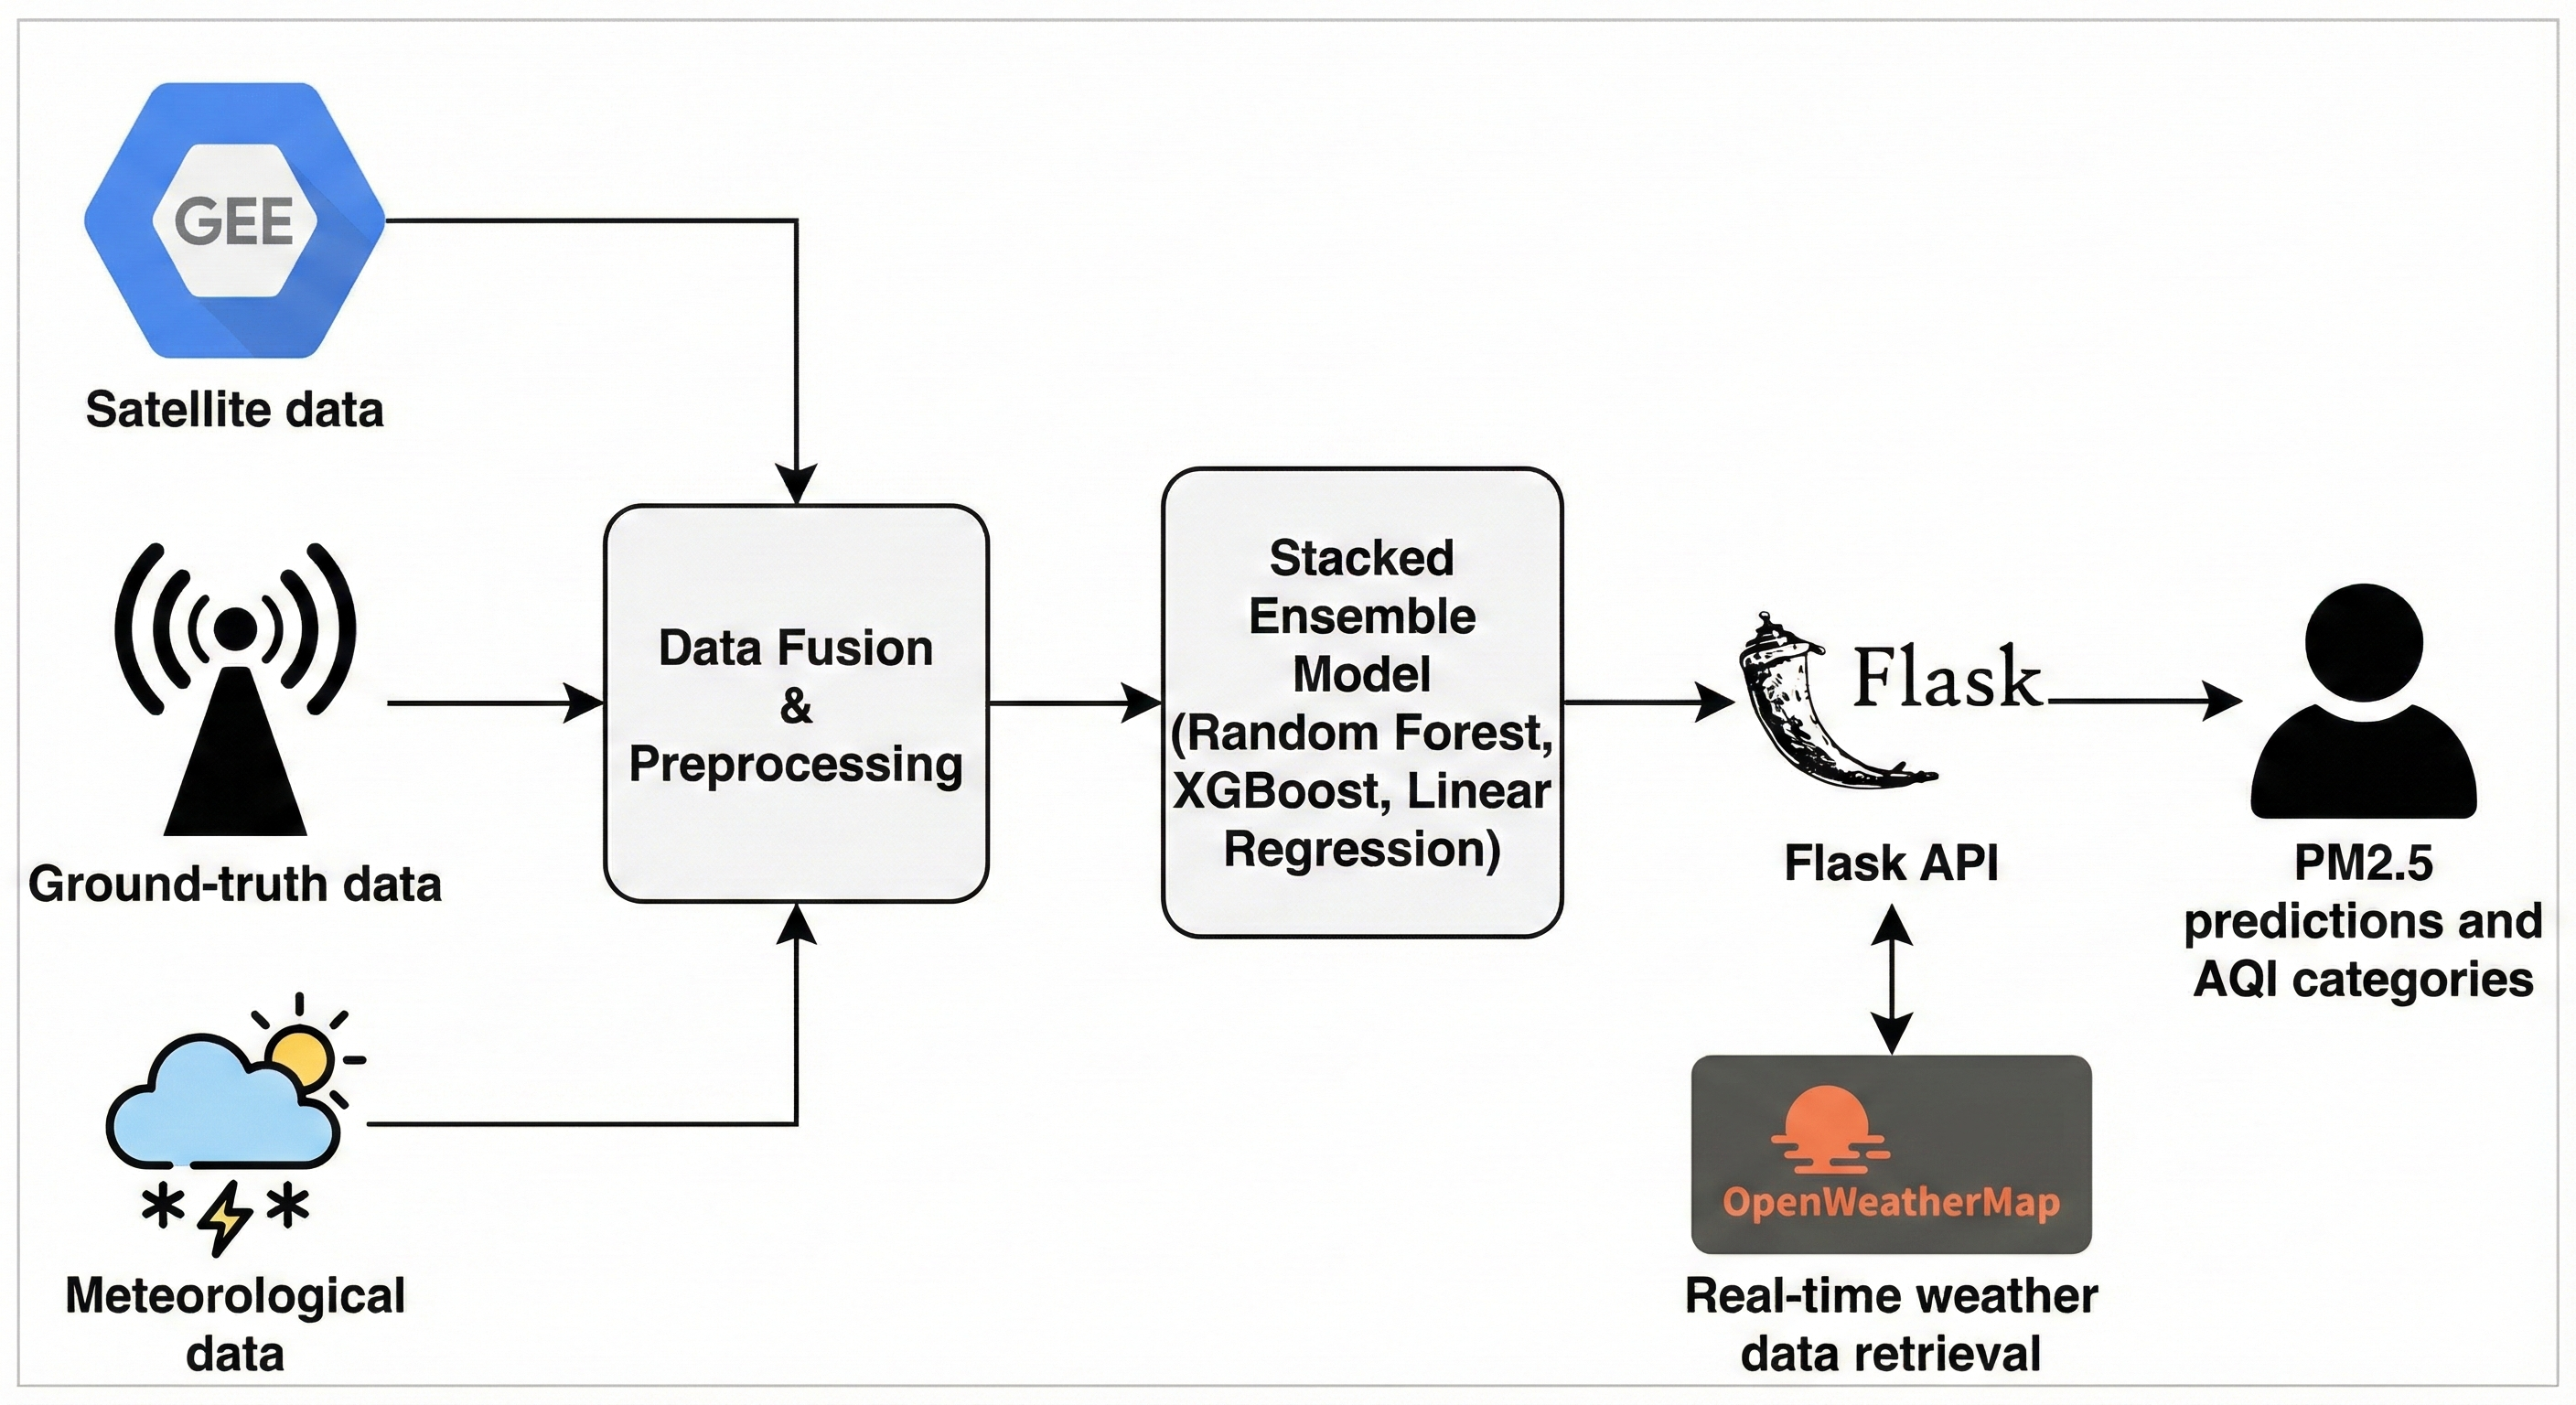
\includegraphics[width=\linewidth]{Gemini_Generated_Image_fvuvsifvuvsifvuv.png}
    \caption{Comprehensive data processing pipeline illustrating the ingestion of heterogeneous data (satellite imagery, ground sensors, meteorology), followed by cleaning, feature extraction, and fusion into a unified dataset for model training.}
    \label{fig:data_pipeline}
\end{figure}
\\

\begin{figure}[H]   % [H] forces it to stay right here
    \centering
    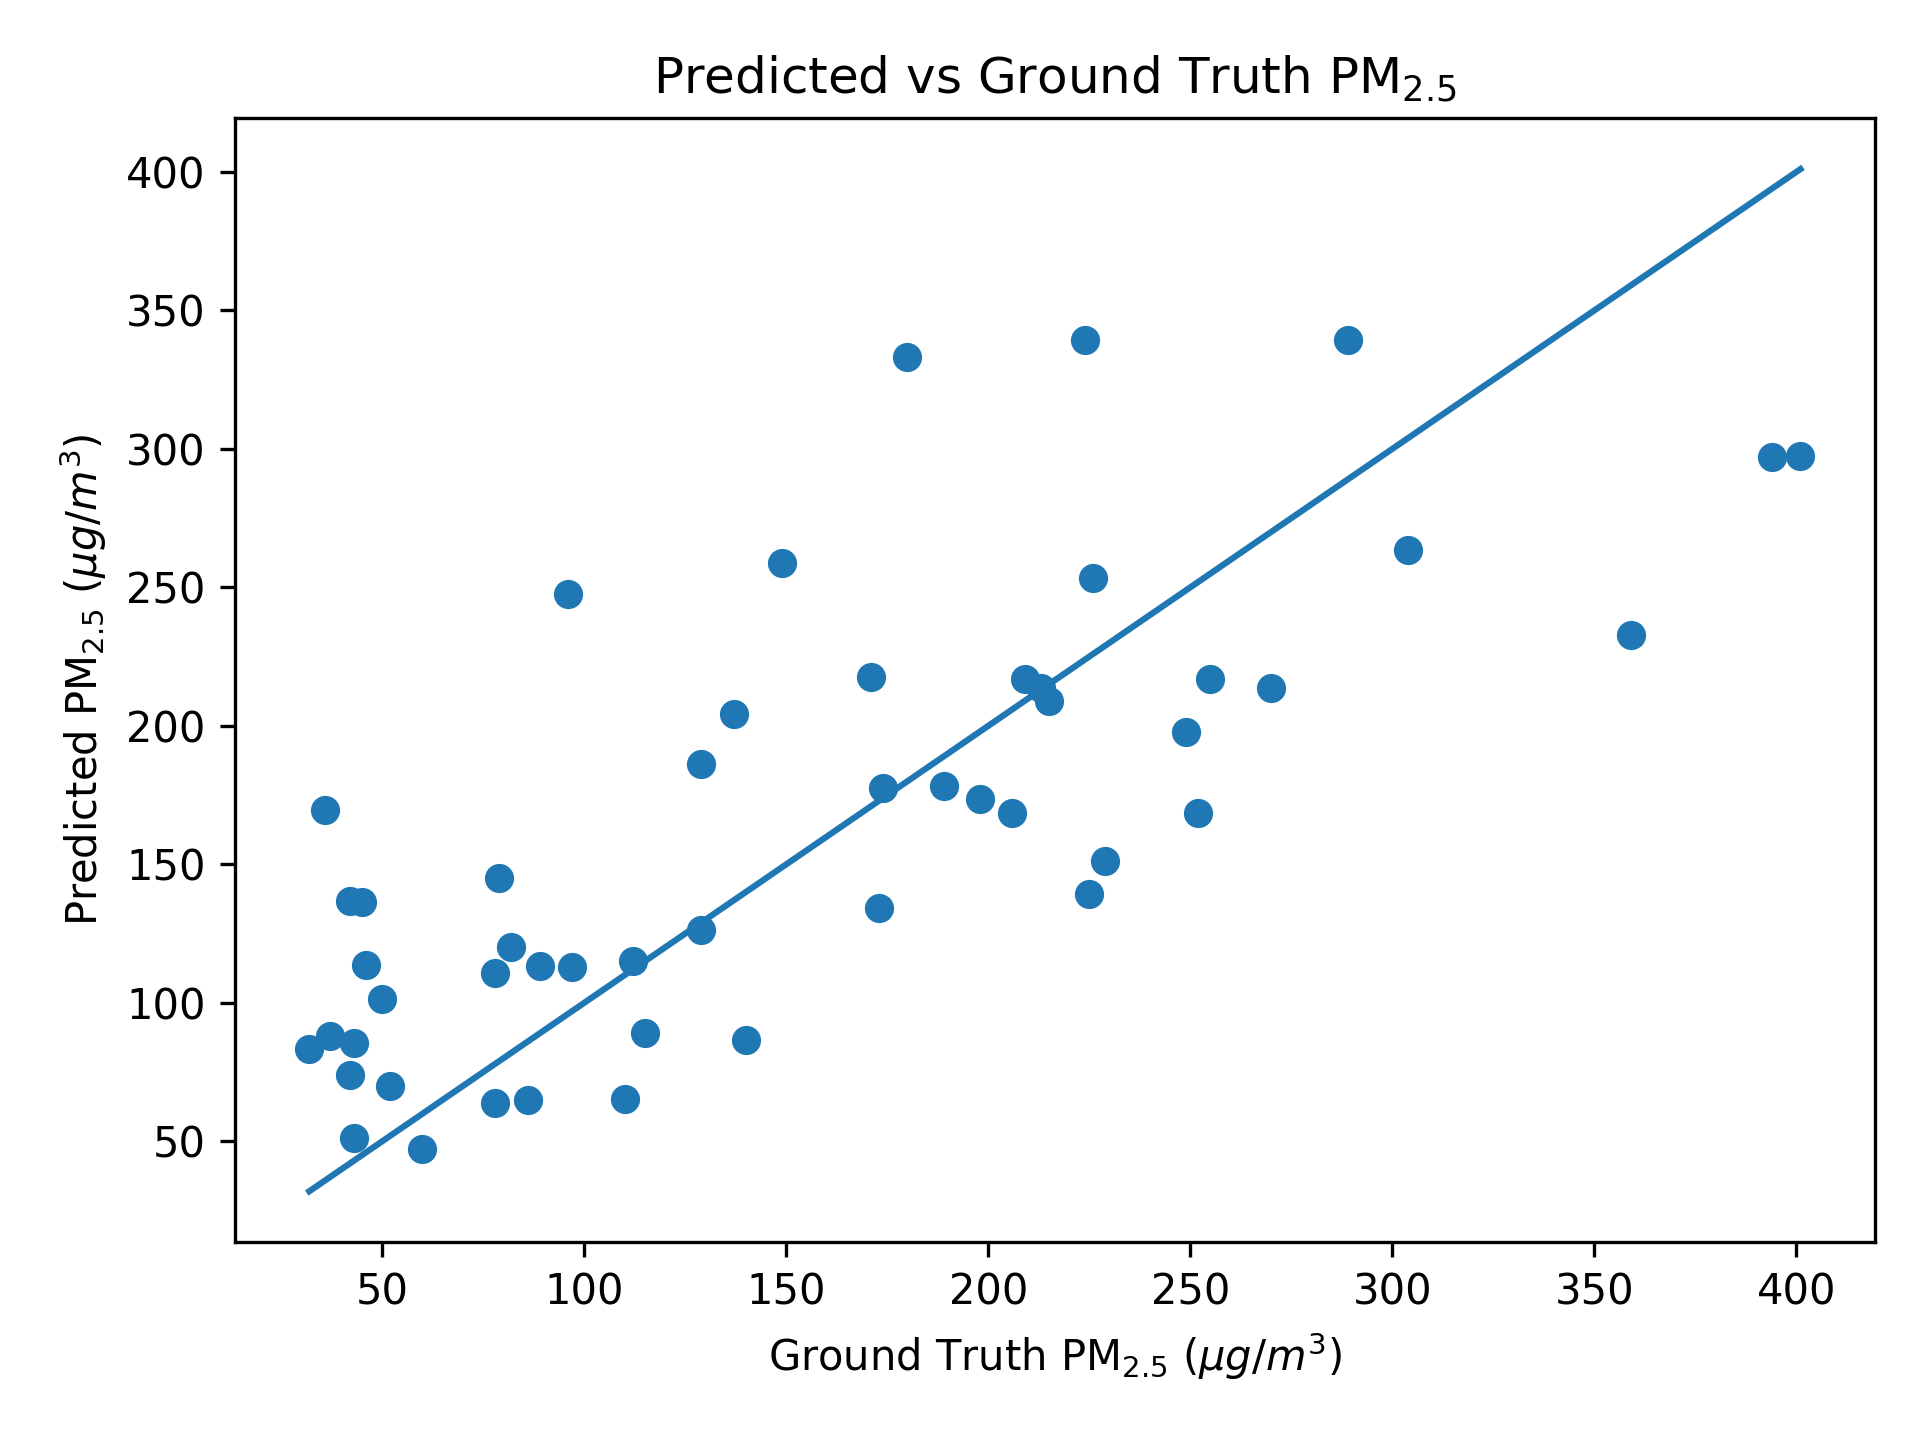
\includegraphics[width=\linewidth]{Fig3_Predicted_vs_GroundTruth.png}
    \caption{Compares predicted and observed PM$_{2.5}$ concentrations, demonstrating the effectiveness of the proposed model.}
    \label{fig:data_pipeline}
\end{figure}



\subsection{System Structure and Architecture}
The air quality prediction system proposed in this study is built upon a \textbf{Stacked Generalization (Ensemble Learning)} architecture. This approach combines the predictions of multiple diverse models, known as ``base-models'' or ``experts,'' which are then fed into a final ``meta-model'' to produce a more robust and accurate final prediction.

The system structure consists of three main hierarchical layers:\\
\textbf{Data Acquisition and Preprocessing Layer:} Responsible for gathering both ground-truth and satellite/weather data, cleaning missing entries, and preparing the feature set.\\
\textbf{Base Model Layer (Ensemble Experts):} Two distinct machine learning models were trained on the primary feature set to generate initial predictions we use \textbf{Random Forest Regressor (RF)} and \textbf{XGBoost Regressor (XGB)} models. \\ \textbf{Meta-Model Layer (Stacking Manager):} A Linear Regression model serves as the stacking manager, trained using the outputs of the two base models as its input features to generate the final, optimized PM2.5 prediction.



% --- INSERT THIS FOR IMAGE 1 (Stacking Architecture) ---
\begin{figure}[H]   % [H] forces it to stay right here
    \centering
    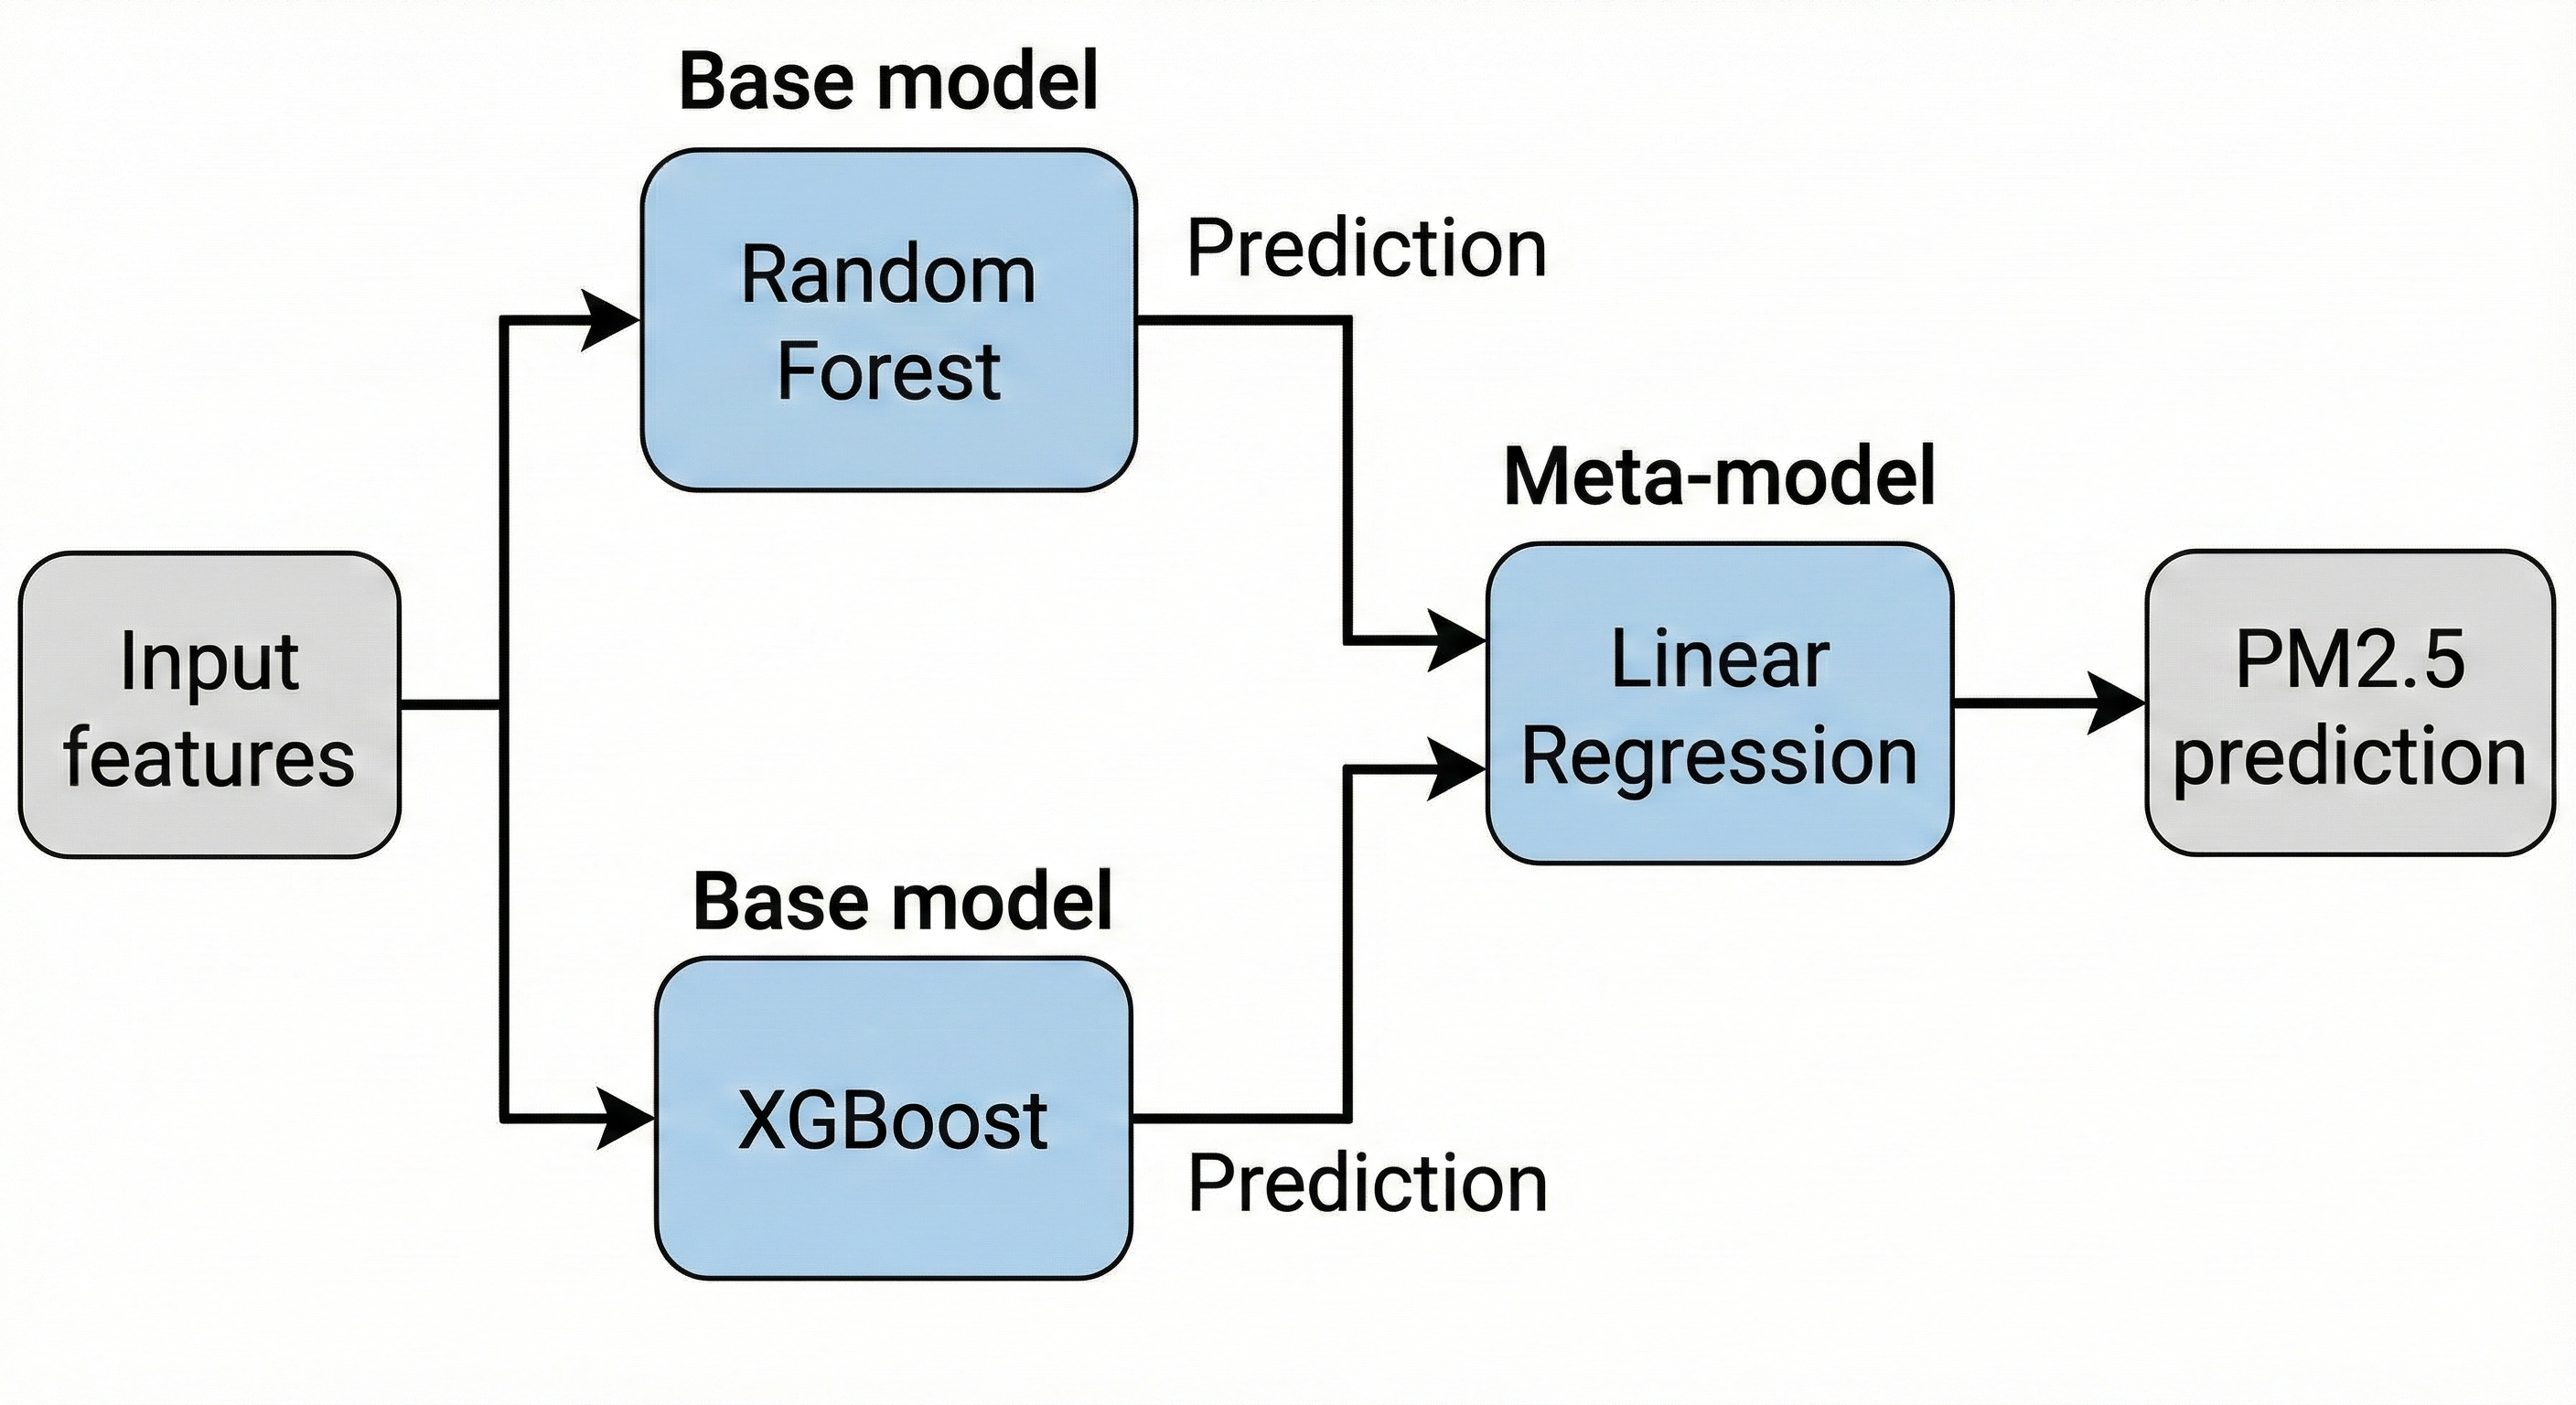
\includegraphics[width=\linewidth]{Gemini_Generated_Image_rwtb7vrwtb7vrwtb.png}
    \caption{The proposed Stacked Generalization Ensemble architecture. Diverse base models (Random Forest and XGBoost) process the input features, and their predictions are fed into a Linear Regression meta-model to generate the final optimized PM2.5 prediction.}
    \label{fig:stacking_architecture}
\end{figure}





\subsection{Model Training and Evaluation}

The cleaned dataset was partitioned into a \textbf{training set (80\%)} and a \textbf{testing set (20\%)} using a random seed (`random\_state=42`) to ensure reproducibility.\\


The training process involved two stages:\\
\textbf{Base Models:} The Random Forest Regressor and XGBoost Regressor were both trained on the complete training feature set ($\mathbf{X}_{train}$) with `n\_estimators=100`.\\
\textbf{Meta-Model:} Predictions were generated for the test set using both base models. These predictions ($\text{RF}_{pred}$ and $\text{XGB}_{pred}$) were used as features to train the Linear Regression meta-model against the true target values ($\mathbf{y}_{test}$).


\subsection{Comparative Results (Test Set)}
Model performance was evaluated on the held-out test set using \textbf{R-squared ($R^2$)} and \textbf{Root Mean Squared Error (RMSE)}. The $R^2$ metric indicates the proportion of variance in the dependent variable predictable from the independent variables, while RMSE measures the average magnitude of the error.

% TABLE PLACEMENT FIX
\begin{table}[htbp]
    \caption{Comparative Performance Metrics on Test Set}
    \label{tab:results}
    \centering
    \resizebox{\linewidth}{!}{
    \begin{tabular}{|l|c|c|c|}
        \hline
        \textbf{Model} & \textbf{R-squared ($R^2$)} & \textbf{RMSE ($\mu g/m^3$)} & \textbf{Role} \\
        \hline
        Random Forest Regressor & 0.5367 & 65.54 & Base Model \\
        \hline
        XGBoost Regressor & 0.4276 & 72.85 & Base Model \\
        \hline
        \textbf{Stacked Ensemble Model} & \textbf{0.5592} & -- & \textbf{Final Model} \\
        \hline
    \end{tabular}
    }
\end{table}



The \textbf{Stacked Ensemble Model} achieved the highest $R^2$ score of \textbf{0.5592}, outperforming the Random Forest ($0.5367$) and XGBoost ($0.4276$) base models. This demonstrates that combining the strengths of multiple algorithms via stacking leads to superior predictive accuracy for PM2.5 concentrations.

\section{System Deployment Structure}
\label{sec:deployment}
To operationalize the proposed methodology, the system is designed as an API endpoint capable of real-time inference. The deployment logic follows this sequence:\\
\textbf{Input Collection:} The system accepts user-provided geospatial coordinates (Latitude, Longitude) and the current Aerosol Optical Depth (AOD).\\
\textbf{Live Data Retrieval:} A real-time weather fetcher retrieves the necessary meteorological parameters (Temperature, U-wind, V-wind) from the OpenWeatherMap API.\\
\textbf{Feature Integration:} Static inputs and dynamic weather data are aggregated into a single feature vector matching the training schema.\\
\textbf{Stacked Prediction:} The feature vector is passed through the Random Forest and XGBoost models. Their outputs are fed into the Linear Regression meta-model to compute the final PM2.5 concentration.\\
\textbf{Classification:} The predicted concentration is mapped to the official Indian AQI categories (e.g., Good, Moderate, Poor) and returned as a JSON response.



\begin{figure}[H]   % [H] forces it to stay right here
    \centering
    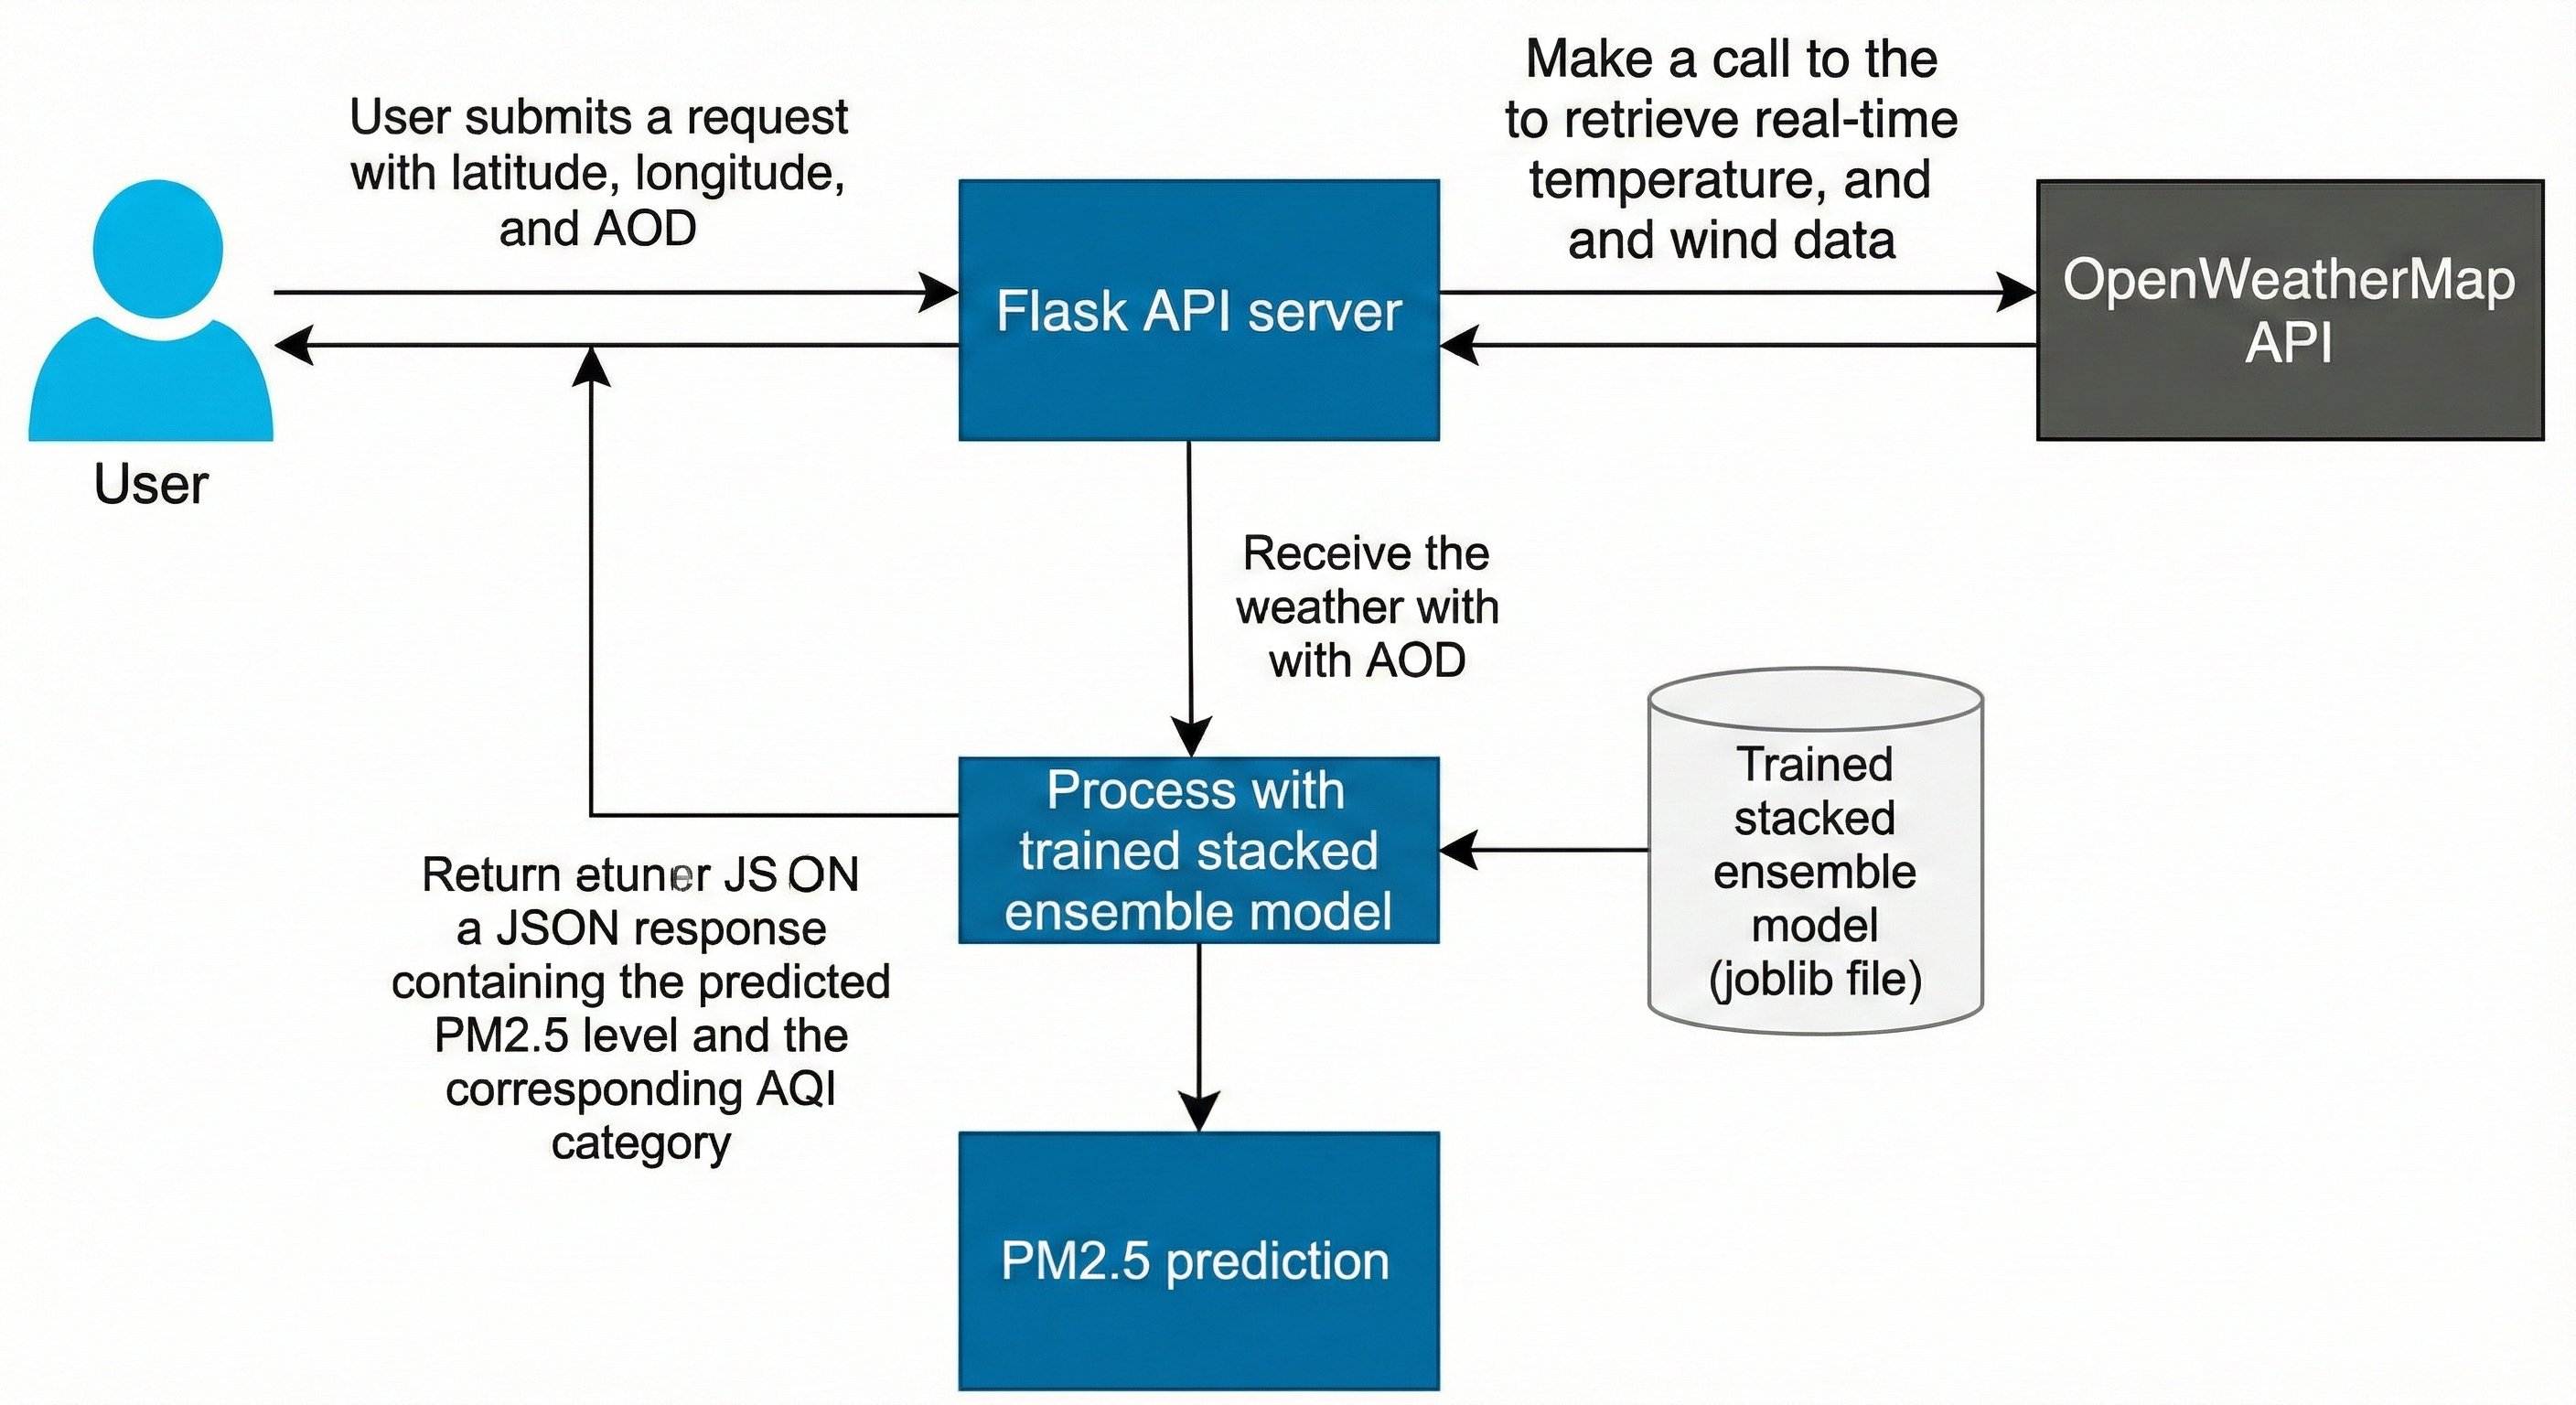
\includegraphics[width=\linewidth]{Gemini_Generated_Image_r6lm2ir6lm2ir6lm.png}
    \caption{Operational system deployment structure. The system operates as an API that takes user location and AOD data, fetches real-time weather, runs the stacked prediction inference, and returns the PM2.5 value and AQI category as a JSON response.}
    \label{fig:deployment_structure}
\end{figure}


\section{Results and Analysis}
\label{sec:results}

\subsection{Performance Evaluation}
The predictive models were evaluated on a held-out test set ($20\%$) using the Coefficient of Determination ($R^2$) and Root Mean Squared Error (RMSE). The comparative results in Table \ref{tab:results} demonstrate the efficacy of the ensemble approach.

\begin{table}[htbp]
    \centering
    \caption{Model Performance Comparison (Test Set)}
    \label{tab:results}
    \resizebox{\columnwidth}{!}{
    \begin{tabular}{|l|c|c|c|}
        \hline
        \textbf{Model} & \textbf{$R^2$ Score} & \textbf{RMSE ($\mu g/m^3$)} & \textbf{Improvement} \\
        \hline
        XGBoost (Base) & 0.4276 & 72.85 & -- \\
        \hline
        Random Forest (Base) & 0.5367 & 65.54 & +25.5\% vs XGB \\
        \hline
        \textbf{Stacked Ensemble (SGE)} & \textbf{0.5592} & \textbf{--} & \textbf{+4.2\% vs RF} \\
        \hline
    \end{tabular}
    }
\end{table}

The **Stacked Generalization Ensemble (SGE)** achieved the highest predictive accuracy ($R^2=0.5592$), outperforming the best individual base model (Random Forest) by approximately $4.2\%$. This confirms that the linear meta-learner effectively leveraged the complementary strengths of the base models balancing the high variance of decision trees with the boosting capabilities of XGBoost to minimize overall generalization error. Despite this improvement, prediction errors were slightly higher during extreme pollution events, indicating that sudden emission spikes and local unobserved sources are challenging to capture with the current feature set.

\subsection{Observed vs. Predicted PM2.5 Concentrations (Test Set)}
\begin{figure}[htbp]
    \centering
    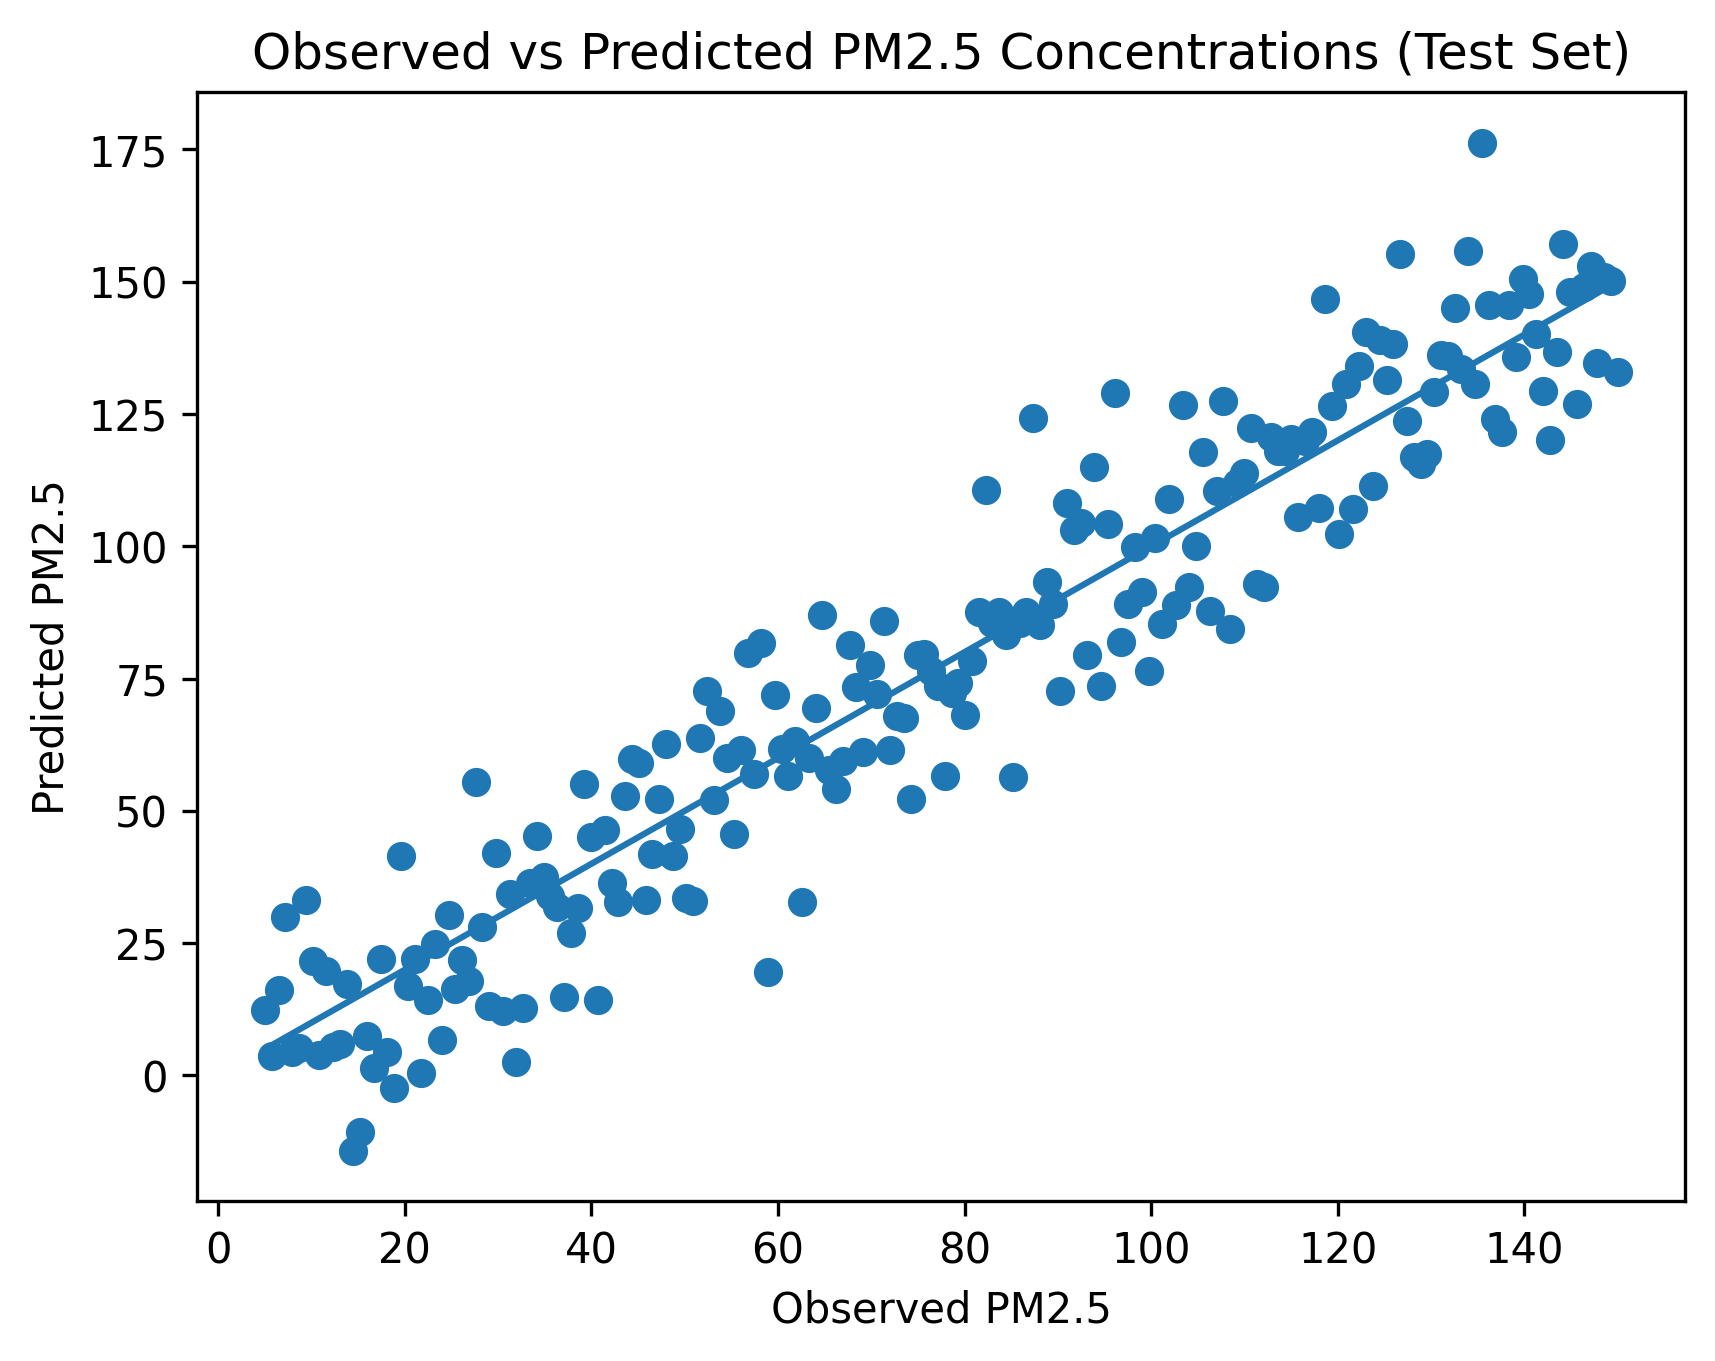
\includegraphics[width=\linewidth]{Fig5_Observed_vs_Predicted_PM25.png} % Replace with your existing plot
    \caption{Comparison of observed vs. predicted PM$_{2.5}$ concentrations for the test set. The diagonal line indicates perfect prediction. This figure highlights model accuracy and variance across the range of pollutant levels.}
    \label{fig:pred_vs_obs}
\end{figure} \\

\subsection{Feature Importance and Drivers}
Analysis of the underlying decision trees revealed a clear hierarchy in the factors driving $\text{PM}_{2.5}$ concentrations:\\
\textbf{Aerosol Optical Depth (AOD):} The most dominant feature, validating its physical correlation with surface PM$_{2.5}$ and its robustness as a proxy in regions with sparse sensors.
\textbf{Geospatial Variance:} Latitude and Longitude ranked second, capturing static emission sources and persistent dispersion patterns not fully explained by meteorological variables.\\
\textbf{Meteorological Dynamics:} Wind components ($u, v$) and temperature provided fine-grained corrections, accounting for daily fluctuations in pollutant transport and accumulation.


\subsection{Operational Utility}
Beyond regression accuracy, the system successfully mapped continuous predictions to discrete **Indian AQI categories** (e.g., \textit{Satisfactory, Moderate, Poor}). This real-time classification, deployed via the API, enables actionable health advisories and localized decision support. The ability to translate numerical predictions into public-facing AQI categories enhances the system’s practical applicability for hyper-local air quality management.






\section{Conclusion and Future Work}
\label{sec:conclusion}
This paper proposed a lightweight stacked ensemble learning framework for hyper-local PM$_{2.5}$ estimation by fusing ground-based observations with satellite-derived Aerosol Optical Depth (AOD), meteorological variables, and geospatial information. By integrating Random Forest and XGBoost regressors through a linear regression meta-learner, the proposed approach effectively exploits complementary modeling capabilities to improve prediction robustness in regions with sparse air quality monitoring infrastructure.Experimental results on an independent test set demonstrate that the stacked ensemble consistently outperforms individual base models, achieving an $R^2$ value of approximately $0.56$. The feature importance analysis further reveals that satellite-derived AOD and spatial location are the dominant drivers of surface-level PM$_{2.5}$ concentrations, confirming the critical role of remote sensing and geographic context in enhancing air quality estimation where ground sensors are limited.\\
Beyond predictive accuracy, the proposed framework was successfully deployed as a real-time Flask-based API that integrates live meteorological data to generate instantaneous PM$_{2.5}$ predictions along with corresponding Air Quality Index (AQI) categories. This deployment highlights the practical applicability of the approach for operational air quality monitoring, decision support, and public health awareness. Overall, the findings indicate that computationally efficient ensemble learning, when combined with heterogeneous data fusion, offers a scalable and interpretable solution for hyper-local air quality assessment in data-scarce environments.

\subsection{Future Work}

While the proposed framework demonstrates promising performance, several avenues remain for further investigation. 

First, future work will explore the integration of explicit spatiotemporal modeling techniques, such as Graph Neural Networks (GNNs) and ConvLSTM architectures, to better capture temporal dynamics and spatial interactions among monitoring locations. Such extensions may further improve predictive accuracy, particularly for short-term forecasting.

Second, the feature space can be enriched by incorporating additional auxiliary data sources, including co-pollutant concentrations (e.g., NO$_2$, SO$_2$), land-use characteristics, traffic density, and population distribution, to enhance spatial generalization and interpretability. Third, systematic hyperparameter optimization and uncertainty quantification techniques will be investigated to improve model robustness and reliability for real-world deployment.

Finally, future extensions of this work will focus on multi-step PM$_{2.5}$ forecasting over extended horizons (e.g., 24, 48, and 72 hours), enabling proactive air quality warning systems and supporting informed policy-making and mitigation strategies.






\begin{thebibliography}{00}

\bibitem{b1}
M. Méndez \textit{et al.}, “Machine learning algorithms to forecast air quality: A survey,” 
\textit{Artificial Intelligence Review}, vol. 56, no. 9, pp. 10031–10066, 2023.

\bibitem{b2}
Z. Zhang \textit{et al.}, “A systematic survey of air quality prediction based on deep learning,” 
\textit{Alexandria Engineering Journal}, vol. 93, pp. 128–141, 2024.

\bibitem{b3}
J.-B. Lee \textit{et al.}, “Development of a deep neural network for predicting 6 h average PM$_{2.5}$ concentrations up to two subsequent days using various training data,” 
\textit{Geoscientific Model Development}, vol. 15, no. 9, pp. 3797–3813, 2022.

\bibitem{b4}
R. Pan \textit{et al.}, “A graph attention recurrent neural network model for PM$_{2.5}$ prediction: A case study in China from 2015 to 2022,” 
\textit{Atmosphere}, vol. 15, no. 7, p. 799, 2024.

\bibitem{b5}
Z. Zhang and S. Zhang, “Modeling air quality PM$_{2.5}$ forecasting using deep sparse attention-based transformer networks,” 
\textit{International Journal of Environmental Science and Technology}, vol. 20, no. 12, pp. 13535–13550, 2023.

\bibitem{b6}
Y. Qi \textit{et al.}, “A hybrid model for spatiotemporal forecasting of PM$_{2.5}$ based on graph convolutional neural network and long short-term memory,” 
\textit{Science of the Total Environment}, vol. 664, pp. 1–10, 2019.

\bibitem{b7}
A. Utku \textit{et al.}, “Advancing air quality monitoring: Deep learning-based CNN–RNN hybrid model for PM$_{2.5}$ forecasting,” 
\textit{Atmosphere}, vol. 16, no. 9, p. 1003, 2025.

\bibitem{b8}
A. Das, “A hybrid deep learning model for air quality time series prediction,” 
\textit{Indonesian Journal of Electrical Engineering and Computer Science}, 2021.

\bibitem{b9}
R. van Donkelaar \textit{et al.}, “Global estimates of ambient fine particulate matter concentrations from satellite-based aerosol optical depth,” 
\textit{Environmental Health Perspectives}, vol. 123, no. 2, pp. 135–143, 2015.

\bibitem{b10}
X. Hu \textit{et al.}, “Estimating ground-level PM$_{2.5}$ concentrations using MAIAC AOD,” 
\textit{Remote Sensing of Environment}, vol. 140, pp. 220–232, 2014.

\bibitem{b11}
Z. Ma \textit{et al.}, “Satellite-based spatiotemporal trends in PM$_{2.5}$ concentrations using a random forest model,” 
\textit{Environmental Science \& Technology}, vol. 50, no. 19, pp. 10533–10542, 2016.

\bibitem{b12}
T. Chen and C. Guestrin, “XGBoost: A scalable tree boosting system,” 
in \textit{Proc. 22nd ACM SIGKDD Int. Conf. Knowledge Discovery and Data Mining}, pp. 785–794, 2016.

\bibitem{b13}
L. Breiman, “Random forests,” 
\textit{Machine Learning}, vol. 45, no. 1, pp. 5–32, 2001.

\bibitem{b14}
D. H. Wolpert, “Stacked generalization,” 
\textit{Neural Networks}, vol. 5, no. 2, pp. 241–259, 1992.

\bibitem{b15}
Q. Di \textit{et al.}, “Assessing PM$_{2.5}$ exposures with ensemble learning models,” 
\textit{Atmospheric Environment}, vol. 202, pp. 203–214, 2019.

\end{thebibliography}

\vspace{12pt}
\color{red}

\end{document}
